\chapter{Distributed Data Aggregation}\label{chap:dda}
\section{Definition}
Data aggregation is a technique that , on its basis, consists in reducing the amount of data collected, reducing the resources needed to process it.  According to \cite{journals/corr/abs-1110-0725}, data aggregation is  considered a subset of information fusion, that aims at reducing the handled data volume. A more precise definition is given in the same report:
\begin{definition} An aggregation function $f$ takes a multiset of elements from a domain $I$ and produces an output of a domain $O$.
\begin{equation*} f : \mathbb{N}^I \to O \end{equation*}
\end{definition}
The order in which the elements are aggregated is irrelevant and a given value may occur several times.
The main goal of data aggregation, "\textit{the aggregation function aims to summarize information. The result of an aggregation takes less space than the inputed multiset (element from $\mathbb{N}^I$)}".\\
Distributed data Aggregation or \textit{in-network} aggregation tends to distribute de computation of an aggregation funtion among several nodes in the network. In contrary of a \textit{centralized} architecture, where a central node compute all the data and performs the aggregation function, a \textit{de-centralized} aggregation distribute the data, hence the effort to compute the aggregation function is reduced.

\section{Wireless Sensor Network}
Wireless Sensor Networks(WSN) are \textit{ad-hoc} networks composed by tiny devices with limited computation and energy capacities. These tiny devices, sensors, are called tiny because of their low capability of computation, communication and storage. The WSN  low-cost sensors monitor physically on environmental conditions, such as temperature, sound, vibration, pressure, monitor pollutants and to cooperatively pass their data through the network to a main location(sink node) via multi-hop wireless links\cite{asad2013survey} or to their peers.\\ 
WSNs act under severe technological constraints: individual sensors have severely limited computation, communication and power(battery) resources and need to operate in settings with great spatial and temporal variability.The ad-hoc nature of a WSN implies that sensors are also used in the network infrastructure, i.e., not just sending their own data and receiving direct instructions but also forwarding data for other sensors. Modern networks are bi-directional, enabling control of sensor activity but some WSN could not have bi-direccional communicatin  due to low computation power of the sensors. The development of wireless sensor networks was motivated by military applications such as battlefield surveillance.\\
Today, WSN networks are used in many industrial and consumer applications like industrial process monitoring and control, machine health monitoring and so on. Some of WSNs requirements are:  large number of nodes, low energy use, network self organization, collaborative signal processing and querying ability.\\
 WSNs are becoming increasingly popular in many spheres of life \cite{castelluccia2005efficient}, they also have the capability of forming the sensor web services which can be considered as an extension of the future internet towards smart devices, Internet of Things(IoT)\cite{asad2013survey}.

\subsection{WSN and Smart Grids}
Considering the overall appliances, WSNs has also several applications in the SG. Furthermore, the AMR could be considered as a specific example regarding the appliance of WSN. It can be implemented the proposed WSN solutions for data aggregation in AMR .\\
Recently, WSN has been widely  recognized as a vital component of the electric power system\cite{journals/ijdsn/Liu12}. WSN contains a large number of low cost and multifuncional sensor nodes which "\textit{can be of benefit to electric system automation application, especially in urban areas}"\cite{RePEc:eee:rensus:v:15:y:2011:i:6:p:2736-2742}. The collaborative and context-awareness nature of WSN brings several advantages over traditional sensing including great fault tolerance, improved accuracy, larger coverage area and extraction of localized features \cite{journals/ijdsn/Liu12}. Sensor nodes can monitor the overall network.\\
WSN could apply to several features in the SG: basis measurement, smart voltage sensors, smart capacitor control, smart sensors for outage detections and weather condition sensors, distributed generation, smart gird storage and, referenced before and more importantly for this work, WSN for AMI( Advanced Metering Infrastructure) or AMR.
A specific example is in \cite{journals/ijdsn/Liu12} where a WSN could apply perfectly to a household or House Area Network(HAN) . ZigBee  is a communication technology often choosed in Smart Grids  due to its reliable wide area coverage and predictable latencies, it is also a suitable choice for a Local Area Network such as a household or a neighborhood. As a example in \cite{journals/ijdsn/Liu12}, a WAMR(Wireless Automatic Meter Reading) can determinate real-time energy consumption of the customers by sensing each device that has a wireless sensor on it. The smart meter within the household perform an interface that translates, summarizes and aggregates data of power usage and presents it to the power utility.\\ 
Other examples of WSN appliances in SG are found in \cite{journals/ijdsn/Liu12}. WSN could apply in Power Delivery and in Power Generation as well since the sensors can monitor the deliver systems, in the first case, and monitor the energy generated in the second case.\\
Although very similar, there are some differences between WSN and Automatic Meter Reading. Such diferences are stated in \cite{khalifa2011survey}. For example, individual consumption measurments must preserve its information. In WSN, sink doesn't care about inidivudal data but in AMR, aggregation nodes must preserve the unique measurments, plus, the meters must have a unique indentifier that links the smart meter to a household/costumer/producer. Futhermore, Smart meters have fixed positions on contrary to some WSN, base stations may need to disconnect/connect to a specific costumer. Even in security, there are some differences. The main security concern in WSN is to preserve the privacy of data, in SM, altough privacy is an important issue, integrety of data is the main concern.\\
WSN, even considering the diferences to AMR, it provides a variety of solutions and gives some insight to understand and comprehend the problem of distributed aggregation in AMR since WSN is a well studied subject.The topology we can find in some WSN can apply to the ones in the AMR. So, even with differents communication infrastrutures or different computation powers,  from the topological view, both networks are very similar.\\

\section{Distributed Data Aggregation Algorithms}
Distributed Data Aggregation Algorithms are protocols used to compute aggregation function in a \textit{decentralized} way. They are used and more suitable when the network lacks a node or component that have the computonational capacitie to process large ammounts of data. The case of WSN , were all the nodes are tiny devices with low storage and proccessing capacity.\\
In \cite{journals/corr/abs-1110-0725} is also presented a simple taxonomy of the existing algorithms that performe distributed data aggregation. First it is analyzed the algorithms from the communication perspective, i. e., the routing protocols and the intrinsic topologies, afterwards, it is analyzed the computation issues, how the aggregation functions are computed by the algorithms.


\subsection{Communication}

\subsubsection{Hierarchy-based approaches} 

Traditionally, existing aggregation algorithms operate on a hierarchy-
based communication scheme. This is \textit{structured} communication scheme. It is required to know in advance the topology of the network. A hierarchy communication tree is constructed, with several levels of nodes. In the root of the tree there is a main repository of all data, denominated as sink. Besides the sink, other special nodes can be defined to compute intermediate aggregates, working as aggregation points that forwards their results to upper level nodes. There are generally two main phases, \textit{request} phase, corresponding to an aggregation request spreading through all the nodes, an the \textit{response} phase where all the nodes respond to the request sending their aggregation results. Some specific examples of these kind of communication are presented.\\
\\
\textbf{\textit{TAG}} The Tiny Aggregation algorithm that suits for ad-hoc networks described in \cite{madden2002tag}. This algorithm requires the previous creation of a tree-based routing topology, and the continuous maintenance of such routing structure in order to operate over mobile networks. TAG provides a SQL-like declarative language to the users. The algorithms consists of two main phases, the \textit{distribution} phase, i which a aggregation query is disseminated through all the spanning tree, and a \textit{collection} phase, where the values are aggregated. A waiting time is required to conclude this two phases.\\
\\ 
\textbf{\textit{DRINA}} DRINA is a cluster based protocol described in \cite{villas2013drina} that denominates the algorithm as \textit{lightweight and reliable routing approach for in-network aggregation in wireless sensor networks}. Considers four roles for each node: textit{colaborator}, a node that detects an event and reports the gathered data to coordinator one,\textit{coordinator} a node that also detects an event and  collected all the gathered data sent by collaborator nodes, aggregating them and sending the result to upper levels,\textit{sink}, a node that receives all the data from a set of coordinators and finnaly a \textit{relay}, a node that just forward the data towards the sink. The algorithm works in three phases: First the hop tree from the sensor nodes to the sink node is built. In this phase, the sink node starts building the hop tree that will be used by Coordinators for data forwarding purposes, second the cluster formation and cluster-head election, third phase is responsible for setting up a new route and updating the hop tree.\\ \\


\textbf{\textit{DAG}} An aggregation scheme fro WSN is proposed in \cite{motegi2006dag} that aims to reduce the number of message losses. For each node, multiple parents are set but only one is chosen to aggregate intermediate values. The most common parent's parent(grandparent) are chosen among the list received as the destination aggregator. Messages are aggregated if the receiving node corresponds to the destination, forwarded if correspond to its parent or discarded otherwise.\\
\\

\textbf{\textit{Sketches}} Algorithm proposed in \cite{considine2004approximate} that uses small sketches. Based on the probabilistic counting sketches technique that estimates the number of distinct elements in a data collection and it is described in further detail in \cite{fan2008efficient}. Like other algorithms of this type, is uses two phases: the sink propagates the aggregation request across the network and then the results are collected back to the sink. In the first phase, all nodes compute their distances to the root, in the second phase the partial aggregates are computed across the routing structure, using the adapted counting sketch scheme, and send to the upper levels in successive rounds.\\
\\
\textbf{\textit{I-LEAG}} Cluster-based aggregation approach designated as I-LEAG is in \cite{birk2006veracity}. The routing structure of this algorithm is composed by a hierarchy of clusters or partitions. A single pivot is designated for each cluster and the root is the pivot of the upper level cluster. This structure can be consider similar as we can see in networks with \textit{super-peers}, but organized in a tree structure. The algorithm works as follows: each cluster check local conflicts that are reported to the pivot, then the pivot computes the new aggregate and multicast the result, each node must forward the received result to the nodes outside the cluster.\\
\\
\textbf{\textit{Tributary-Delta}} 
This approach mixes the traditional use of tree and multi-path routing schemes, dividing the network in two routing regions: \textit{delta}(multipah) and \textit{tributary}(tree). Use tributaries in regions with low rate of message losses to take advantage of traditional tree schemes and delta in regions with higher rate of message losses(mostly regions near the sink with the aggregate of several nodes).

\subsubsection{Gossip-based approaches}
This type of approach is referred as an \textit{unstructured} approach, contrary of the aforementioned \textit{structed} approaches. In this type of scheme there is no previous knowledge of the topology of the network or any specific structure. The information or messages are commonly disseminated across the network without following any specific topology, the information it is passed node to node, or nodes, like a infectious disease or a gossip,i.e., an "infected" node sends a message to a random subset of nodes. This type scheme tends to allow a robust(fault tolerant) and scalable information dissemination all over the network\cite{journals/corr/abs-1110-0725}\\
\\
\textbf{\textit{Push-Sum Protocol}}  Push-sum protocol is described in \cite{kempe2003gossip} and it is a gossip-based protocol. \cite{journals/corr/abs-1110-0725} describes the algorithm function : along discrete times $t$, each node $i$ maintains and propagates information of a pair of values $(s_ti,w_ti)$ where $s$ represents the sum of the exchanged values and $w$ the weight associated. In each iteration, a neighbor is chosen uniformly at random and half of the actual values are sent to the target node and the other half to the node itself. Upon received, the local values are updated, adding each value from a received pair to its local component.

\subsubsection{Hybrid approaches} 
Hybrid approaches propose a solution that merge both hierarchic and gossip-based approaches, using the high accuracy and efficiency of the hierarchic based schemes and the robustness of the gossip approaches. In the disadvantages of one approach , the other one has it as an advantage, Hybrid approaches aim to merge the advantages of both schemes to eliminate both disadvantages.\\
\\
\textbf{\textit{Chitnis et al, 2008}} Chitnis et al.\cite{chitnis2008aggregation} proposed an hybrid approach, using TAG as an hierarchy-based approach and Push-Sum as a gossip-based protocol. This hybrid approach divides the network node in groups. Inside each group, a gossip-based protocol is used. In each group, a leader is elected to further perform a hierarchic communication with other  leaders nodes regarding the aggregation results from the gossip group. 

\subsection{Computation}
\subsubsection{Hierarchical}
The input is separated into groups so it can be computed in a distributed hierarchical way.  It depends on the previous formation of a communication structure such as tree or cluster. Some node work as \textit{forwarders}, just forward data to upper levels of the hierarchy, and others work as \textit{aggregators}, apply the aggregation function directly to all received input and then works as a normal \textit{forward} node. This class of algorithms allows any decomposable function with high accuracy without the presence of faults. Algorithms of this class were aforementioned.
\subsubsection{Averaging}
This class of computation scheme is based on an iterative computation of partial aggregates, where all nodes share their results among the network and all of them contribute for the final result. This scheme provides high accuracy, considering that all nodes converge to the same result.However, in order to converge to the correct result, the algorithms must respect an important principle commonly designated as "mass conservation". \cite{journals/corr/abs-1110-0725} describes "mass conservation" as an invariant, stating that the sum of the aggregated values of all network nodes must remain constant along time. One example of algorithms of this class, is the ones with gossip base communication scheme, since the results of the aggregates could be share randomly with the neighbor nodes. Due to its nature, Averaging algorithms tend to be highly robust, i.e., tolerant to faults on opposite of the structured algorithms. Decomposable and duplicate sensitive functions can be be computed in this class.\\
\\
\textbf{\textit{Push-Pull Gossiping}} Similar to the aforementioned \textit{push-sum protocol}, the push-pull gossiping\cite{jelasity2004epidemic} performs an averaging process. This algorithm executes an epidemic protocol to perform a pari-wise exchange of aggregated values among neighbor nodes\cite{journals/corr/abs-1110-0725}. In periodic intervals of time, a node send its value to a randomly selected node and waits to receive a result back, the response from the selected node. Afterwards, an average with the new value and the present value its performed in order to calculate and store a new one. When a node receives a value from another node, the same process is performed, send the current value and calculate a new one from the average of the received value and the current one.\\ 
\\
\textbf{\textit{DRG(Distributed Random Grouping)}} This approach \cite{chen2006robust} randomly creates groups across the network in which aggregates are successfully computed. There are three modes a node can perform:\textit{leader,idle} and \textit{member} which corresponds to three phases. First every node is in \textit{idle} mode, then every node broadcasts a Group Call Message, pretending to be a group leader(with a pre-defined probability associated ) and waits for members. The nodes who receives the group call, responds to the first one received with a JACK(Joining Acknowledgment) tagged with their aggregated value becoming a member of the group. Finally, the \textit{leader} gathers all the aggregated values, computing the aggregation function($AVERAGE$) and broadcasts a Group Assignment Message with the  final result. Every group member waits until it receives the result from the leader to update its local value and then returns to  \textit{idle} mode.\\
\\
\subsubsection{Sketches}
Algorithms based on the use of an auxilary data structure with a fixed size that holds a \textit{sketch} of all network values. Input values are used to create \textit{sketches} that aggregated across the network, using specific operations to update and merge them. The aggregation could be done using multiple paths. This type of algorithms enables operations of order and enables duplicate insensitive. The computational cost of this class depends mainly on the resources used to produce the result by the estimator and the complexity of the operations to produce the \textit{sketches}. This kind of algorithms tend to be very fast, depending on the dissemination protocol used to propagate the sketches, but lack accuracy because they are based on probabilistic methods.\\
\\
\textbf{\textit{RIA-LC/DC}} Algorithm proposed in \cite{fan2008efficient}, a multi-path routing aggregation approach. The algorithm consists of two phases. First an aggregation request is sent by the sink throughout the whole network, creating a multi-path routing hierarchy. Second, starting in the lower levels, each node generates a \textit{sketch} correspondent to its current state and sends it to the nodes in the upper level. The node that receives the \textit{sketch}, creates a new one combining tis current value and the received \textit{sketch} and sends it to the upper node until the top is reached where the sink computes the aggregation estimate.\\
\\
\textbf{\textit{Extrema propagation}}
This approach reduces the computation of an aggregation function\cite{journals/corr/abs-1110-0725}. A vector $x_i$ of $k$ random number is created at each network node $i$. Random numbers are generated according to a known random distribution, using the node initial value as an input parameter. The execution of the algorithm \textit{"consists of the computation of the point wise minimum between all exchanged vectors"}\cite{journals/corr/abs-1110-0725}. At each node, the obtained vector is used as a sample to produce an approximation of the aggregation result. This algorithm is focused on obtaining a fast estimate, rather than an accurate one. 
\subsubsection{Digests}
This class of algorithms allowd the computation of more complex functions like median or mode than the normal aggregation function such as $SUM$ or $AVERAGE$. This algorithms produces a \textit{digest}, data structure with a bounded size that holds an approximation of the statistical distribution of input values in the whole network, that summarizes the system data distribution, an histogram. The accuracy of this class of algorithms depends mostly on the quality and size of the obtained \textit{digest}. Usually it requires more resources.\\
\\
\textbf{\textit{Q-Digest}} This aggregation scheme allows the approximation of complex aggregation function in WSN is proposed in \cite{shrivastava2004medians}. It uses an hierarchical routing topology to build and disseminate quantile digests. Each node maintains a quantile digest of the data availabe, which is built in a button-up fashion by merging received digest from lower nodes(children nodes). This new quantile digests are compressed according to a specific compression factor. Aggregation functions are computed by manipulating and traversing the quantile structure according to a specific criteria.\\
\\
\textbf{\textit{Equi-Depth}} Gossip-based approach described in \cite{horowitz2003estimating}. The scheme executes a gossip protocol and merges specific function on the exchanged data. Each node keeps a list of $k$ value or \textit{digests}, initially set to its input value. Each node randomly chooses a neighbor to exchange the digest to merge with its own. This round is executed several number of times, producing an approximation of the network distribution of values. There are four merging techniques \textit{swap, concise, equi-with histograms} and \textit{equip-depth histograms} that are detailed in \cite{journals/corr/abs-1110-0725}.\\
\\
\textbf{\textit{Adam2}}
Adam2 is a gossip based algorithm to estimate the statistical distribution of values across a decentralized 
system\cite{sacha2010adam2}. Each node can decide to start an instance of Adam2 where each instance is uniquely identified by its starting node. The starting node $i$ initializes the interpolation set $H_i$(composed of $k$ pairs of values $(x_k,f_k)$ where $x_k$ represents an interpolation point and $f_k$ the fraction of nodes with value less or equal to $x_k$). The interpolation is initialized by setting $f_k$ to 1 if the node attribute reading $v_i$ is less or equal than the corresponding interpolation value $x_k$, 0 otherwise. Node stores a set of interpolation points for each running algorithm instance. A new node that, learning about the new instance, performs a initialization and then starts participating in the protocol. The sets are exchanged like push-pull, the sets are merged by averaging the fraction at each interpolation point. After a predefined number round the CDF is approximated by interpolating the point of the resulting set.
\\
\\
A overall taxonomy table is presented in \cite{journals/corr/abs-1110-0725}

\begin{figure}[h]
\centering
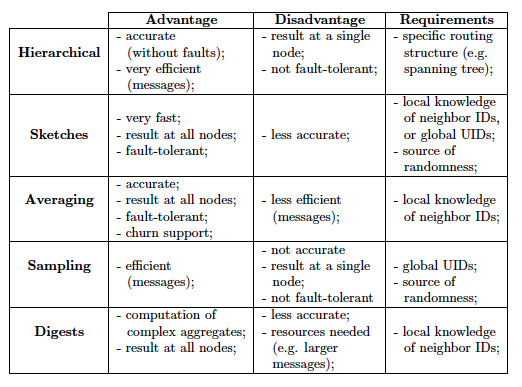
\includegraphics[width=0.75\textwidth]{/Users/rafaelremondes/UM/MEI/Thesis/DistributedAggregationAlgortihmsSM/Writing/Images/tableComp}
\caption{\label{fig:TableTax} Summary of the characteristics of main data aggregation classes}
\end{figure}

\section{Distributed Data Aggregation in WSN}
Distributed Data Aggregation in WSN is an widely study subject, with several works and proposed solutions. Distributed aggregation adquires a special importance in WSN, since the sensor are low resources devices so the effort distribution is quite mandatory. The aggregation techniques reduce the amount of data communicated within a WSN and thus conserve battery power \cite{castelluccia2005efficient}.Periodically, as measurements are recorded by individual sensors, they are been collected and processed to produce data representative of the entire WSN.  An natural approach is consider that the sensor send the measured data to special sensor nodes, i.e., aggregator nodes \cite{castelluccia2005efficient}. In \textit{in-network} aggregation nodes forward the aggregated data to a sink that store it.\\
\begin{figure}[h]
\centering
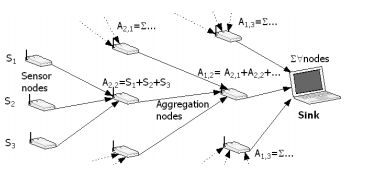
\includegraphics[width=0.5\textwidth]{/Users/rafaelremondes/UM/MEI/Thesis/DistributedAggregationAlgortihmsSM/Writing/Images/INA}
\caption{\label{fig:INAaggregation} Principle of in-network aggregation}
\end{figure}
An example of \text{in-network} aggregation in WSN is in  \cite{castelluccia2005efficient}. In this model, it is assumed that all nodes are potential aggregators and that data gets aggregated as they propagate towards the sink. The aggregation is set as an obligation of being simple not involving any expensive or complex computation. The aggregation requires all sensors to send their data to the sink within the same sampling period so there is a need for a global so that all node can synchronize. Another study is in \cite{Girao2004c}, where a special kind of distributed aggregation is proposed, \textit{Concealed Data Aggregation}. This type of aggregation is defined as an approach than promises the combination os end-to-end security and \textit{in-network} aggregation. In \cite{chan2006secure} it is assumed a general multi-hop network with a set $S={s_1....s_n}$ of $n$ sensor nodes anda a single base station $R$. The aggregation is performed over an \textit{aggregation tree} which is the directed tree formed by the union of all the paths from the sensors nodes to the base station. Another WSN distributed aggregation scenario is presented in \cite{yu2009distributed}. The network model consist of a $n$ sensor nodes and one base station that is also called a sink. Each sensor node can send or receive data to or from all directions. It is assumed that all nodes have the same transmission range for simplicity. A node can either receive or send data at a time and it can receive a data packet correctly when it hears only this packet at that moment.


\section{Smart Metering Aggregation Model} 
There are two main architectures for smart metering considering data aggregation  are \textit{centralized} and \textit{distributed} or \textit{ decentralized}\cite{journals/spm/ErkinTLP13}. In \textit{centralized} fashion, the meters just sense the data, afterwards, it is sent to a central aggregator with higher computation power that holds a central database. In a \textit{decentralized} way, the aggregation role is distributed among several meters, not all of then. This type of aggregation is also called  \textit{in-network} aggregation \cite{Girao2004c}\cite{Castelluccia05efficientaggregation}. The aggregation node in this scheme communicate the calculated energy consumed to an appropriate party such as a energy producer. Typically, this communication occurs once per billable period \cite{journals/spm/ErkinTLP13}. As introduced before, the architecture chosen for this work is \textit{de-centralized} due to the nature of the aggregation algorithms.\\
Several examples of SG projects and models were given in chapter \cite{chap:sg}. Usually, the \textit{centralized} approach is composed by a cloud service provided to the costumers to store their consumption data. These approaches make use of a data center and uses this architecture so they are capable of storing  big quantities of data and perfome Big Data techniches on it, providing useful information for both energy companies and costumers. \\
One example of the \textit{de-centralized} architecture for aggreagation is in the PowerMatching City of Hoogkrek. Because the goals are different than providing statistycall information regarding the costumers consumption, in this case the goal if forming a market in microgird that enables the household to be self-sufficient in therms of energy. They use the \textit{de-centralized} archictecture to form several points of this market wherer households sell and buy their energy, the nodes that concentrates the offers communicate with each creating  the city energy market. Another example is in Rottondi  \textit{et al}\cite{rottondi2012}, the overall scheme is presented in \ref{fig:meterArchitecture}, where a set of meters are connected to gateway sharing information, the central station only works to set the aggregation rules.
\begin{figure}[h]
\centering
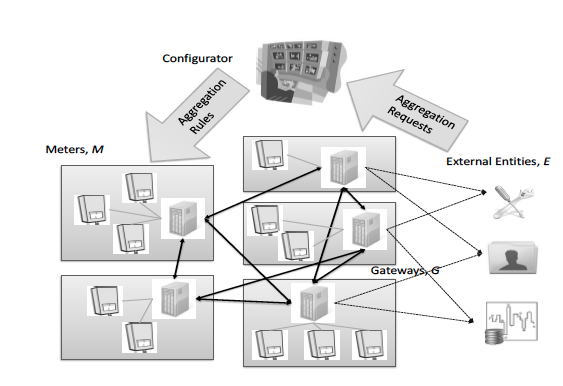
\includegraphics[width=0.5\textwidth]{/Users/rafaelremondes/UM/MEI/Thesis/DistributedAggregationAlgortihmsSM/Writing/Images/meterExample}
\caption{\label{fig:meterArchitecture} The functional nodes of the architecture}
\end{figure}




